\documentclass[12pt]{article}
\usepackage[spanish]{babel}
\selectlanguage{spanish}
\usepackage[utf8]{inputenc}
\usepackage{vmargin}
\usepackage{graphicx}
\setmargins{2.5cm}{1.5cm}{16.5cm}{23.42cm}{0pt}{1cm}{0pt}{2cm}
\title{Iniciando Fortran}
\author{Martín Alejandro Paredes Sosa}
\date{Febrero 2015}
\graphicspath{{IMG/}}

\begin{document}

\maketitle

\section{Introducción}
En esta práctica se inicio a trabajar con \textbf{FORTRAN}, escribiendo algunos comandos y programas sencillos. Estos  nos permiten entender la sintaxis y así poder saber como utilizar los comandos de Fortran.
\\ \\
En el siguiente documento se mostraran los trabajos que se realizaron durante esta actividad así como los resultados de ejecutar estos programas.
\section{Actividades Realizadas}

A continuación se mostraran los programas que se realizaron durante esta actividad.
\\
Se mostraran con el siguiente formato:

\begin{itemize}
\item Descripción del programa
\item El código en Fortran
\item Una imagen de la ejecución del programa
\end{itemize}

\pagebreak

\subsection{Programa: Área del Circulo}

En este programa se pide al usuario que proporcione el radio del circulo con el cual se realizaran los cálculos de la circunferencia y área del circulo.
\begin{verbatim}
!=======================================
! Area.f90 : Calcula el area del circulo
!=======================================

program Area_Circulo !Inicio de programa

  Implicit None
  Real *8 :: radius , circum , area !Declaracion de variables
  Real *8 :: PI = 4.0*atan(1.0)
  Integer :: model_n =1
  print *, 'Ingrese radio' !Hablar con el usuario
  read *, radius !Leer respuesta de usuario
  circum = 2.0*PI*radius !Calculo de la circunferencia
  area = radius*radius*PI !Calcula el area
  print *, 'Programa Número =', model_n
  print *, 'Radio =', radius
  print *, 'Circunferencia =' , circum
  print *, 'Area =', area

end program Area_Circulo
\end{verbatim}

Ejecución del Programa
\begin{center}
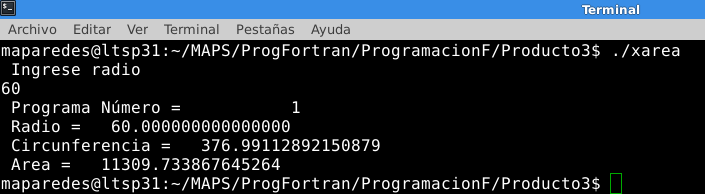
\includegraphics[width=15cm]{Area}
\end{center}

\pagebreak

\subsection{Programa: Volumen}
Este programa es muy similar al pasado en que se pide al usuario que ingrese datos. Lo que se obtiene  con este programa el volumen de liquido contenido en un cuerpo .

\begin{verbatim}
!=======================================
! Volumen.f90 : Calcula el volumen de una esfera
!=======================================

program Volumen_Esfera !Inicio de programa

  Implicit None
  Real *8 :: radius , altura , vol , P3 !Declaracion de variables
  Real *8 :: PI = 4.0*atan(1.0)
  Integer :: model_n =1
  print *, 'Ingrese radio' !Hablar con el usuario
  read *, radius !Leer respuesta de usuario
  print *, 'Ingrese altura' !Hablar con el usuario
  read *, altura !Leer respuesta de usuario
  P3= 3.00 * radius - altura
  vol= 1.00 / 3.00 * PI * altura * altura * P3   !Calculo del volumen
  print *, 'Programa Número =', model_n  !Muestra los resultados obtenidos
  print *, 'Radio =', radius
  print *, 'Altura =' , altura
  print *, 'Volumen =', vol

end program Volumen_Esfera
\end{verbatim}

\begin{center}
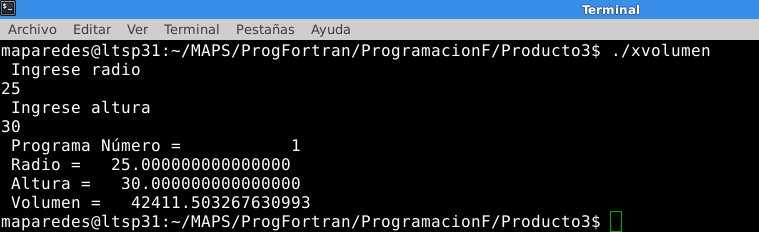
\includegraphics[width=15cm]{Volumen}
\end{center}
\pagebreak

\subsection{Programa: Precisión}
Con este programa se puede apreciar que tan preciso son los cálculos que se obtienen. En este caso es un código de doble precisión.
\begin{verbatim}
!=====================================================
! Precision.f90 : Determina la precision de la maquina
!=====================================================
program Limits
  Implicit None
  Integer :: i , n
  Real *8 :: epsilon_m , one
  n=60 !Establish the number of iterations 
  ! Set initial values : 
  epsilon_m= 1.0
  one= 1.0
  ! Within a DO~LOOP, calculate each step and print .
  ! This loop will execute 60 times in a row as i is
  ! incremented from 1 to n ( since n = 60) : 
  do i= 1,n,1 ! Begin the do~loop
     epsilon_m = epsilon_m / 2.0 !Reduce epsilon_m
     one = 1.0 + epsilon_m ! Recalcular one
     print *, i , one , epsilon_m ! Imprimir los valores
  end do ! End loop when i > n
end program Limits
\end{verbatim}

\begin{center}
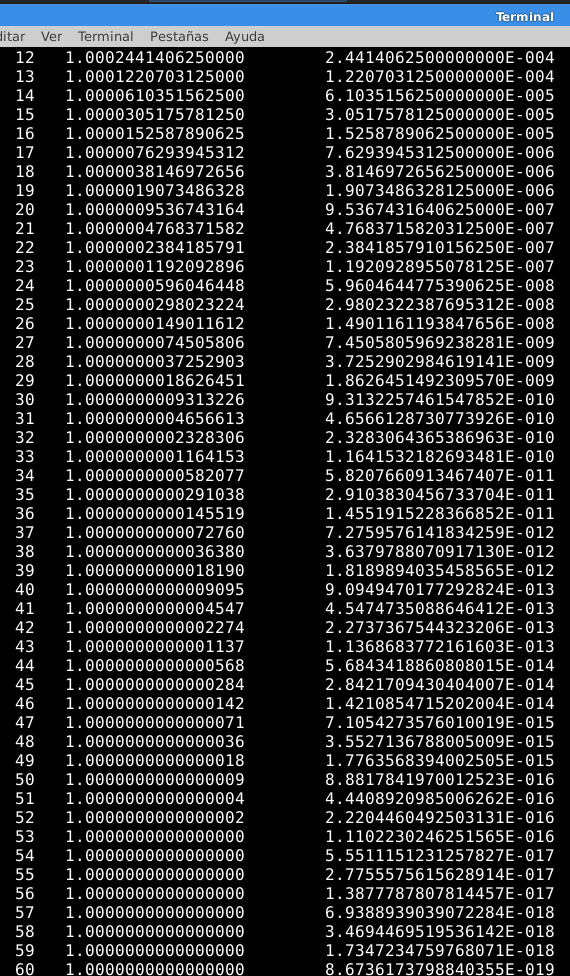
\includegraphics[width=9cm, height =11cm]{Precision}
\end{center}
\pagebreak	

\subsection{Programa: Precisión 2}
Mismo programa que el anterior con la diferencia de que los cálculos son menos precisos (menos decimales) debido a la forma en que declararon los variables.
\begin{verbatim}
!=====================================================
! Precision2.f90 : Determina la precision de la maquina
!=====================================================
program Limits
  Implicit None
  Integer :: i , n
  Real *4 :: epsilon_m , one
  n=60 !Establish the number of iterations 
  ! Set initial values : 
  epsilon_m= 1.0
  one= 1.0
  ! Within a DO~LOOP, calculate each step and print .
  ! This loop will execute 60 times in a row as i is
  ! incremented from 1 to n ( since n = 60) : 
  do i= 1,n,1 ! Begin the do~loop
     epsilon_m = epsilon_m / 2.0 !Reduce epsilon_m
     one = 1.0 + epsilon_m ! Recalcular one
     print *, i , one , epsilon_m ! Imprimir los valores
  end do ! End loop when i > n
end program
\end{verbatim}
\begin{center}
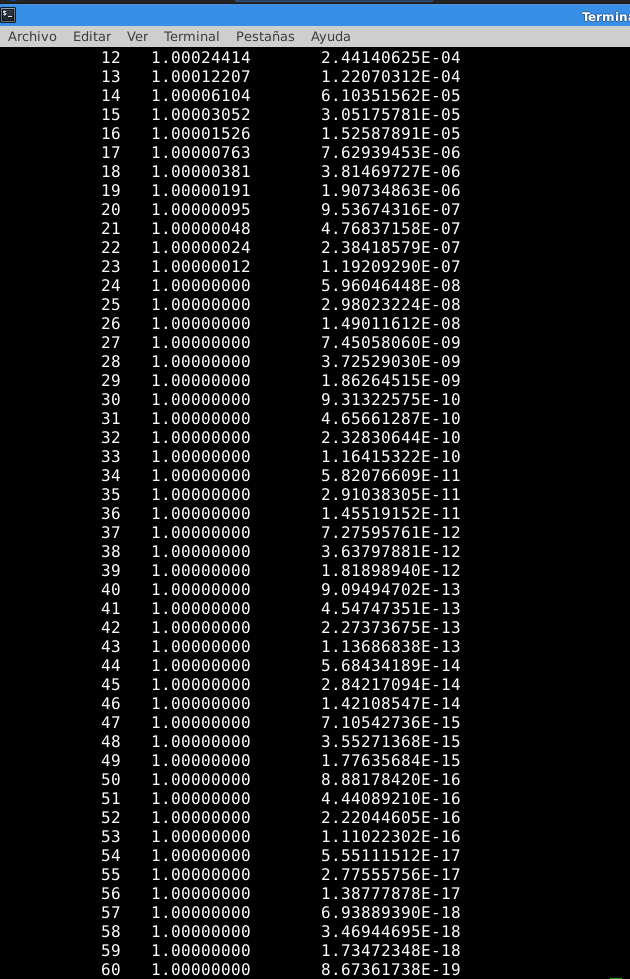
\includegraphics[width=9cm, height=11cm]{Precision2}
\end{center}
\pagebreak

\subsection{Programa: Math}
El lenguaje Fortran maneja funciones trigonométricas y las especiales. Lo que se realizo fue evaluar diferentes funciones e imprimir el resultado.
\begin{verbatim}
!==================================================
! Math.f90 : Desmostracion de funciones matematicas
!==================================================

program Math_Test
  
  Real *8 :: x= 1.0 , y , z
  y= sin (x)
  z= exp (x) + 1.0
  print *, x , y , z
  
end program Math_Test
\end{verbatim}
\begin{center}
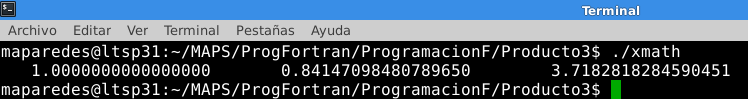
\includegraphics[width=15cm]{Math}
\end{center}

\subsection{Programa: Math 2}
Este programa es muy parecido al anterior con la diferencia a que se evalúan otras funciones que tienen resultados que no son reales.
\begin{verbatim}
!==================================================
! Math2.f90 : Desmostracion de funciones matematicas
!==================================================

program Math_Test

  Real *8 :: x= -1 , y=2.0 , z=0
  Real *8 :: xx , yy , zz
  xx= sqrt (x)
  yy= acos (y)
  zz= log (z)
  print *, xx , yy , zz 
  
end program Math_Test
\end{verbatim}
\begin{center}
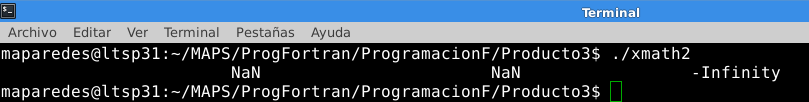
\includegraphics[width=15cm]{Math2}
\end{center}
\pagebreak

\subsection{Programa: Función}
En este programa se declaro un función fuera de lo que es el programa principal con el propósito de poder utilizarla esta función múltiples veces si tener la necesidad de declarar todo de nuevo.
\begin{verbatim}
!===================================
! Funcion.f90 : Llamar a una funcion
!===================================

Real *8 Function f (x,y)
  Implicit None
  Real *8 :: x , y
  f= 1.0 + sin (x*y)
end Function f
!
Program Main
  
  Implicit None
  Real *8 :: Xin =0.25 , Yin= 2 , c , f 
  c = f ( Xin, Yin )
  write ( * , * ) 'f(Xin, Yin) =' , c

end Program Main

\end{verbatim}
\begin{center}
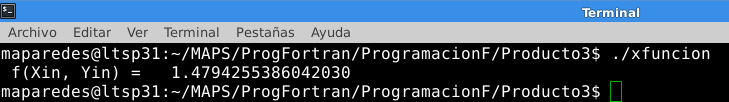
\includegraphics[width=15cm]{Funcion}
\end{center}
\pagebreak

\subsection{Programa: Subrutinas}
Las subrutinas son pequeños programas que son llamados por el programa principal para realizar ciertas acciones, lo que permite que el trabajo sea mas limpio y fácil de manipular.
\begin{verbatim}
!===================================================
! Subrutinas.f90 : Demustra el llamado de subrutinas
!===================================================
Subroutine g(x, y, ans1 , ans2 )

  Implicit None
  Real (8) :: x , y , ans1 , ans2
  ans1= sin (x*y) + 1
  ans2= ans1**2

end Subroutine g
!
program main_program
  
  Implicit None
  Real *8 :: Xin=0.25 , Yin=2.0 , Gout1 , Gout2
  call g(Xin, Yin, Gout1, Gout2 ) 
  write ( * , *) 'The answere are: ' , Gout1 , Gout2

end program main_program

\end{verbatim}
\begin{center}
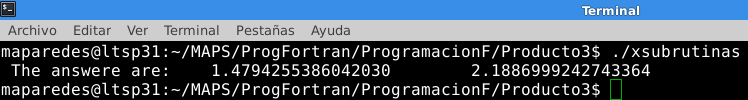
\includegraphics[width=15cm]{Subrutinas}
\end{center}
\end{document}
